\subsection{High level test benches}

The toplevel implementation has four test benches verifying its behaviour.
Like the other test cases these tests are self testing, but a passing test only 
indicates that the result is correct, not that the method of getting there was. 
Hence these tests are harder to verify and are described more in
detail in the following sections. For all the tests a small program is loaded 
into the instruction memory with data loaded into the data memory before the 
processor is enabled for a period of time. 

\subsubsection{Toplevel}
This test bench implements a small, simple program which executes loads, stores, 
adds, ors and ends with a beq instruction which results in a infinite loop.
This test shows the use of most of the implemented instructions, and is quite
large. At the same time it is easy to follow, and we therefore refer the reader
to the screenshot in the attached archive aswell as the actual test bench implementation.

\subsubsection{Branch} 
\label{section:branch-tb}
The branch test bench loads two values into registers and performes four 
conscutive adds. The adds have a data dependecy on the loaded values so the 
first add instruction stalls.
This can be seen when the stall signal goes high in cycle four of figure \ref{fig:branch_tb}.
\begin{figure}[h]
        \centerline{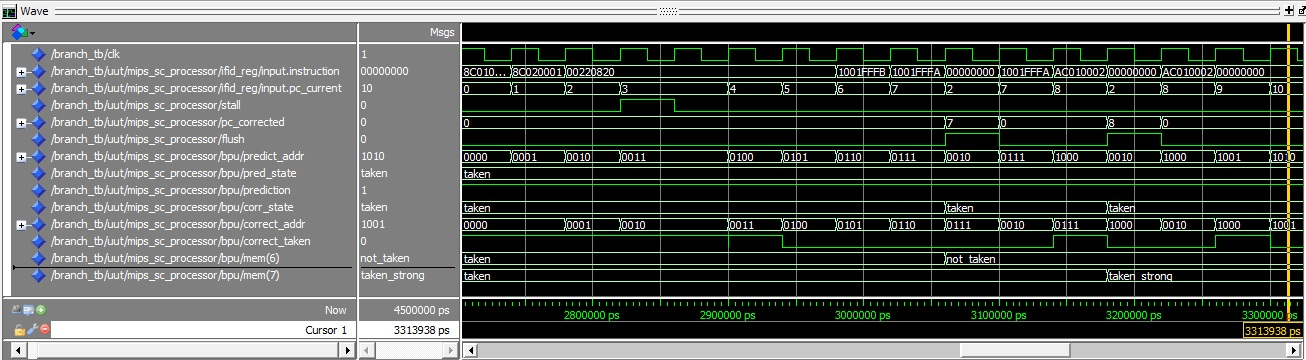
\includegraphics[width=600px]{figures/tb/branch}}
        \caption{The branch test bench}
        \label{fig:branch_tb}
\end{figure}
\FloatBarrier
In cycle 8 (when the \emph{pc\_current} signal is 6) the first branch is fetched from
instruction memory. In the next cycle the second branch is loaded into fetch,
but the branch prediction unit predicts the first branch loaded to be taken. 
As a result the flush signal is pulled high in cycle 9, and the pc changes to
2 in cycle 10.
During cycle 10 the first branch reaches execute, and it is detected that the
branch prediction was wrong. This could have been seen by the correction flush
signal being pulled high, but sadly this signal is missing in the screenshot.
At cycle 11 we're back to instruction 7, the second branch. 

This time the BPU also predicts taken, as seen by the flush. And by cycle 13 
the pc is back to 2. The second branch which now is in execute is evaluated,
and again the prediction was wrong. And in cycle 14 the 8th and final instruction
is loaded.

As mentioned earlier our BPU uses a learning algorithm. The two states for
the two tested branches are shown in the figure. After learning that the first
branch was to be skipped the state changes from TAKEN to NOT\_TAKEN as expected.
However, after the second branch has been evaluated its state changes to TAKEN\_STRONG,
which is wrong. We would expect both of them to end in state NOT\_TAKEN. 
This is caused by a bug in the prediction logic that was not fixed before the deadline.
The bug is not fatal however, as it will only cause some predictions to be sub-optimal.

\subsubsection{For} 
\label{section:for-tb}
This test bench program is a simple for loop, which loops from 1 to 5 before 5 is
written to the data memory. The three constants start, increment and limit are 
initially loaded from data memory.
The loop consists of a branch equal, a add and finally a jump. For each jump taken we
have to flush the if stage, as can be seen by the flush flag. The first time the branch
is evaluated it is predicted taken, as this is the default prediction. But after that one
time it is always predicted not taken, as can be seen by the predict taken signal. During
the last loop the branch is predicted not taken but in fact it should have been taken.
This can be seen by the correction flush close to the end, which clears the IF and ID stages.

This test is a perfect test for our branch predictor as well as forwarding and hazard units
as there are multiple branches, jumps and data hazards. In addition
this testcase is a perfect program to use as a comparison between our two MIPS
implementations. In figures~\ref{fig:for_tb} and ~\ref{fig:multi_cycle_for_tb}, the test output of the test run on both our architectures is shown.

\begin{figure}[h]
        \centerline{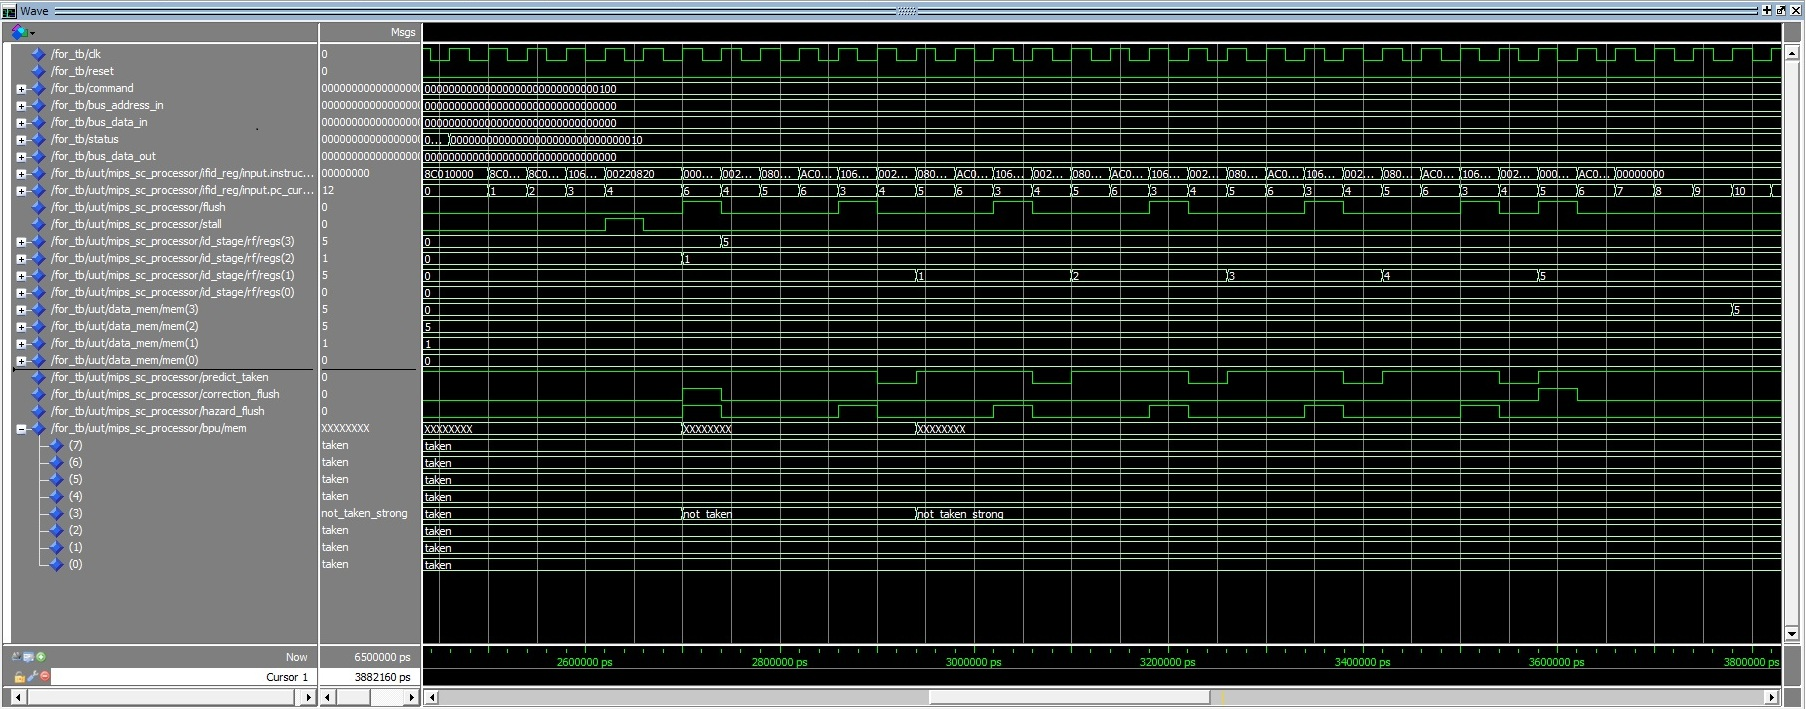
\includegraphics[width=590px]{figures/tb/for_tb2}}
        \caption{For test on pipelined implementation}
        \label{fig:for_tb}
\end{figure}

\begin{figure}[h]
        \centerline{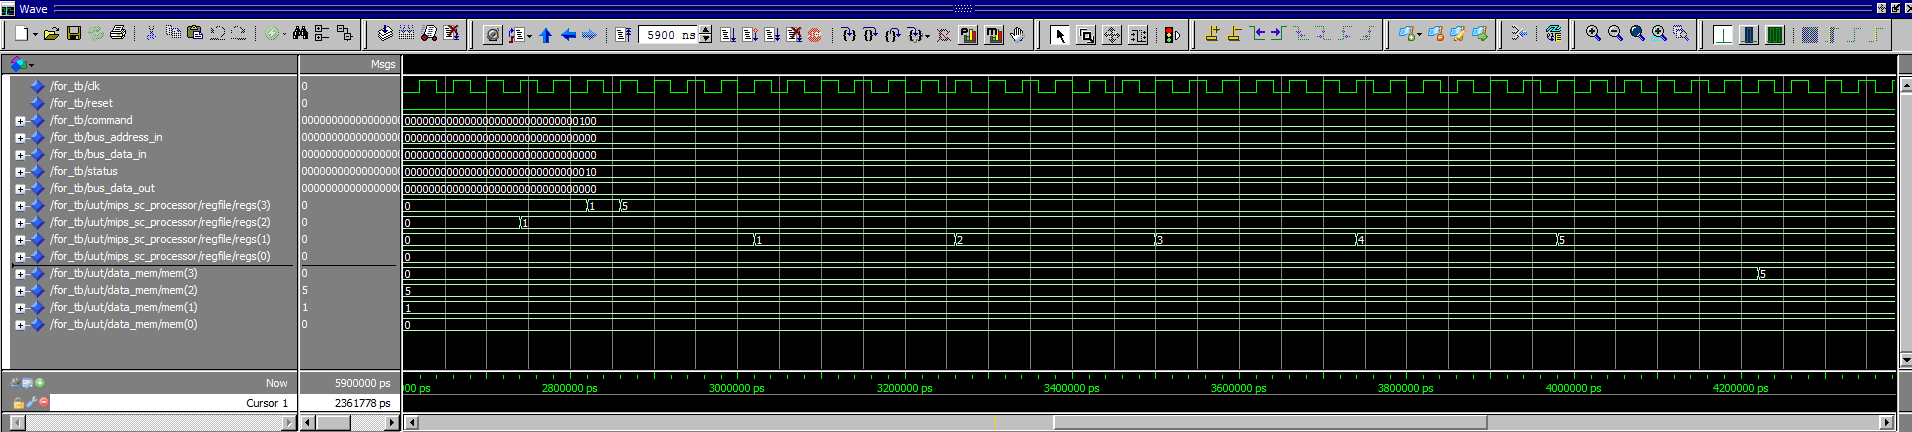
\includegraphics[width=590px]{figures/tb/multicycle_for_test}}
        \caption{For test on multicycle implementation}
        \label{fig:multi_cycle_for_tb}
\end{figure}

As can be read from the two test bench screenshoots, the multicyle
design needs 44 cycles to complete the test while the pipelined design only needs
33 cycles (from the first instruction starts until data is available in memory). 
\FloatBarrier